\documentclass[../notas medios.tex]{subfiles}

\begin{document}
\chapter{Conceptos Preliminares}

\graphicspath{{img/Cap1/}}

\section{Introducción}
En esta sección se presentan las hipótesis básicas que permiten construir el modelo del medio continuo. Dicho modelo debe entenderse como una propuesta ingenieril para abordar problemas de mecánica de sistemas de infinitas partículas usando como herramienta matemática las ideas de continuidad matemática propuestas en el cálculo diferencial.

Al final de esta sección el estudiante debe estar en la capacidad de:
\begin{itemize}
\item[•] Entender el paso de variables discretas a variables continuas en términos de densidades.
\item[•] Identificar la diferencia entre el concepto de partícula en el modelo de la mecánica Newtoniana y el concepto de punto material en el modelo del continuo.
\item[•] Identificar las funciones fuente o causa y efecto o respuesta en el modelo del continuo.
\item[•] Identificar los límites de aplicabilidad del modelo del continuo.
\end{itemize}

\section{Concepto de densidad generalizada}
A una escala de tamaño lo suficientemente pequeña la materia goza de una composición molecular/atómica/microestructural o, en general, de carácter discreto. Lo anterior significa que un volumen finito de material no es otra cosa que una gran colección de partículas, sean estas moléculas, átomos, partículas subatómicas o cualquier otro ente discreto.

Si para esta colección se desea calcular la distribución en el tiempo de alguna función {\bf respuesta} o {\bf efecto} $\beta$ resultante de la consideración de alguna función {\bf causa} $\alpha$, será entonces necesario resolver un sistema acoplado de ecuaciones diferenciales ordinarias tan grande (en número de ecuaciones) como partículas posea la colección. Este sistema de ecuaciones es obtenido a partir de algún principio físico fundamental, conectando las funciones $\alpha$ y $\beta$, y postulado a partir de observación experimental. En términos generales es posible escribir este principio como en la \cref{ca_ef},
\begin{equation}
f\left(\frac{d\beta}{dt} \right) = \alpha\, ,
\label{ca_ef}
\end{equation}
en la cual $\beta$ es la cantidad física que experimenta cambios en el
tiempo y que denominaremos en lo que sigue como función {\bf flujo}, mientras que $\alpha$ es la cantidad física que genera los cambios y la denominaremos la función {\bf interacción}.

Por ejemplo, en el problema mecánico la \cref{ca_ef} correspondería a la segunda ley de Newton en cuyo caso identificamos $\alpha  \equiv \vec F$, siendo $\vec F$ la fuerza actuante sobre una partícula de masa $m$ y $\vec \beta  \equiv m\vec V$  la cantidad de movimiento asociada con la velocidad $\vec V$ de esta partícula.  En este caso $f$ estaría definida como  $f(x)=x$ para un argumento $x$.

Por tanto, si se dispone de un postulado físico fundamental como el dado en
la \cref{ca_ef}, la determinación de las funciones flujo $\beta$ para cada una de las partículas es simplemente una tarea operativa.  Sin embargo, la gran cantidad de partículas de las cuales puede estar compuesto el sistema hacen que este tratamiento ``exacto” a nivel discreto sea imposible de realizar en términos prácticos.  Es decir, la posibilidad de una solución exacta al problema se encuentra limitada por razones operacionales o computacionales. En términos prácticos es válido considerar el volumen finito de material como un sistema de infinitas partículas para cuya solución se requiere tratar con infinitas ecuaciones diferenciales ordinarias.  Este planteamiento puede entenderse como la pregunta o problema general que se busca resolver mediante un {\bf modelo} de los medios continuos. Este busca una solución práctica al problema de calcular una distribución de funciones flujo, debidas a unas interacciones en un sistema de ``infinitas” partículas.

Un tratamiento aproximado se hace posible gracias a la Hipótesis Básica de Continuidad Matemática.  Esta encuentra su motivación en el carácter continuo que soporta el espacio matemático; entre dos puntos, sin importar que tan cercanos se encuentren, siempre es posible encontrar otro punto. Se tiene, entonces,  la definición clásica de continuidad matemática o concepto de límite y en la cual el punto podría definirse a partir de una celda volumétrica $\Delta V$ cuyo tamaño se reduce por un proceso de paso al límite
\begin{equation}
\mathop {\lim }\limits_{\Delta V \to 0} \Delta V = \text{Punto}\, .
\label{lim_point}
\end{equation}

La generalización de este concepto al sistema de infinitas partículas se reduce a despreciar el carácter discreto de la materia y asumir que estas se encuentran distribuidas en el espacio matemático de manera continua, es decir, esta generalización equivale a afirmar que las infinitas partículas ocupan un volumen finito sin dejar vacíos ni discontinuidades entre las mismas. En lo que sigue denominaremos esta distribución físicamente ficticia {\bf El Continuo Físico}. En otras palabras la celda de volumen $\Delta V$  independientemente de su tamaño siempre estará compuesta del mismo material ya que se ha despreciado completamente todo ente micro-estructural.

Podemos en este punto precisar el objetivo fundamental de un modelo de los medios continuos:
\begin{quote}
Un modelo de los medios continuos pretende estudiar la distribución espacio-temporal de las interacciones  y flujos   resultantes en un sistema discreto de infinitas partículas que es aproximado mediante un proceso de promediado basado en la hipótesis básica de continuidad y por ende, convirtiendo las variables involucradas a nivel discreto en campos o distribuciones.
\end{quote}

\section{Conexión entre el continuo físico y el continuo matemático}
Retomando el tratamiento del problema de determinación de una función {\bf
respuesta} $\beta$ para un sistema de muchas partículas sometidas a algún tipo de {\bf excitación} externa o {\bf interacción} $\alpha$, es
claro que, desde el punto de vista operativo, es imposible resolver las ecuaciones
resultantes (discretas) para un sistema de infinitas partículas, por lo que es necesario recurrir a la hipótesis de continuidad matemática con dos consecuencias inmediatas:
\begin{itemize}
\item Se renuncia al concepto de partícula.
\item Se hace disponible la potente herramienta del continuo matemático o
cálculo diferencial.
\end{itemize}

Por ejemplo, en el caso de la mecánica de los medios continuos no tendrá sentido
hablar términos como ``la fuerza aplicada a una partícula” en el sentido discreto. 
Más aún, en las ecuaciones gobernantes a nivel del continuo este concepto mismo de fuerza discreta desaparece matemáticamente y es necesario utilizar representaciones equivalentes que tengan significado dentro del contexto de los medios continuos, es decir funciones, como en este caso la función tensorial de tensiones.

La hipótesis de continuidad genera entonces un modelo que producirá resultados correspondientes a una aproximación con respecto a una solución discreta \footnote{Si se asume que el resultado que se obtendría de un modelo discreto en caso de ser este.}. El orden del error en la aproximación, será siempre relativo y estará fuertemente ligado a la relación entre el tamaño característico del espécimen en cuestión y el tamaño característico de la micro-estructura que se ha despreciado.  Por ejemplo, considere el caso de una viga de concreto.  En ésta, la menor dimensión característica del espécimen correspondería al espesor $h$ mientras que la mayor dimensión característica de la micro-estructura seria el diámetro del agregado grueso $\phi$.  La aproximación introducida al asumir el medio como un continuo físico dará errores despreciables siempre que $h \gg \phi$.  En la medida en que $h \to \phi$   la contribución del agregado a la interacción mecánica es relevante y el modelo del continuo se vuelve impreciso.

El hecho de renunciar al concepto de partícula y de apelar al continuo matemático implica que toda variable de tipo discreto o asociada al concepto de partícula es tratada ahora como una distribución o función.  Replanteando en estos términos y por segunda vez el objetivo fundamental de un modelo de los {\bf Medios Continuos} este se debería reescribir como sigue:
\begin{quote}
Un modelo de los medios continuos pretende estudiar la variación espacio-temporal de las distribuciones o funciones de {\bf respuesta} (o efecto) debidas a una distribución espacio-temporal de funciones {\bf fuente} (o causa).
\end{quote}

En el caso particular del problema {\bf Mecánico} el interés es describir la
respuesta del sistema en términos de {\bf cantidad de movimiento}.  En este escenario las fuentes corresponden a fuerzas o mejor aún, a distribuciones de fuerzas.  Más concretamente, una vez introducida la hipótesis de continuidad, el objetivo será el de determinar funciones continuas representativas de la cantidad de movimiento en respuesta a funciones representativas de las fuentes o fuerzas.

Se puede afirmar entonces que el carácter infinito del sistema de partículas genera la necesidad de un modelo matemático para describir ahora la interacción \footnote{En el caso mecánico una fuerza no es otra cosa que la representación equivalente de una interacción entre dos sistemas.} entre 2 sistemas.  Uno de los sistemas es el medio continuo en cuestión (sistema de muchas partículas) que interactúa o en el caso mecánico intercambia cantidad de movimiento con otro sistema externo.  Denominaremos este (otro medio continuo) como el medio ambiente \footnote{Cadavid, J (2009).  Mecánica del Medio Continuo Una Iniciación.  Fondo Editorial Universidad EAFIT.}.

\section{Características generales de un modelo del medio continuo}
Para apoyar el análisis considérese un medio infinito ocupando un volumen $B(t)$
y que representa en este caso el medio ambiente, \cref{infinite}. Este medio se
encuentra acotado por una superficie ${S_\infty }$ localizada a una distancia infinita de cualquier punto del medio.  Consideramos además un medio continuo ({\bf el sistema}) ocupando un volumen $V(t)$ y localizado al interior de este espacio infinito.  La interfase entre el sistema y el medio ambiente corresponde a una superficie $S(t)$ \footnote{En la \cref{infinite} la frontera del medio continuo representada por $S$ podría ser por ejemplo la de una viga, una presa o si se quiere tan solo una frontera matemática.}. Las preguntas que nos proponemos responder son:

\begin{itemize}
\item ¿Cómo describir la interacción o intercambio de cualquier variable física
del tipo {\bf respuesta} entre el medio (ambiente) infinito  $B(t)$ y el medio continuo $V(t)$ debido a una distribución de variables de tipo {\bf fuente} o {\bf causa}?
\item ¿Cómo expresar esta interacción como una función continua, es decir
llevada a nivel del punto matemático como se hace en el cálculo diferencial?
\end{itemize}

Con referencia a la \cref{infinite} utilizaremos la siguiente descripción de las regiones involucradas.  La región localizada del lado positivo del vector normal ${\hat n^{( + )}}$ a $S(t)$ se denominará en lo que sigue la {\bf región externa}.  De manera consistente, la región localizada del lado negativo del vector normal ${\hat n^{( - )}}$ a $S(t)$ se denominará la {\bf región interna}.  Deseamos entonces caracterizar la interacción entre las regiones interna y externa debida a la existencia de una fuente localizada ya sea sobre $B(t)$ o sobre  $V(t)$. Además queremos describir esta interacción como una función continua.
\begin{figure}[H]
\centering
	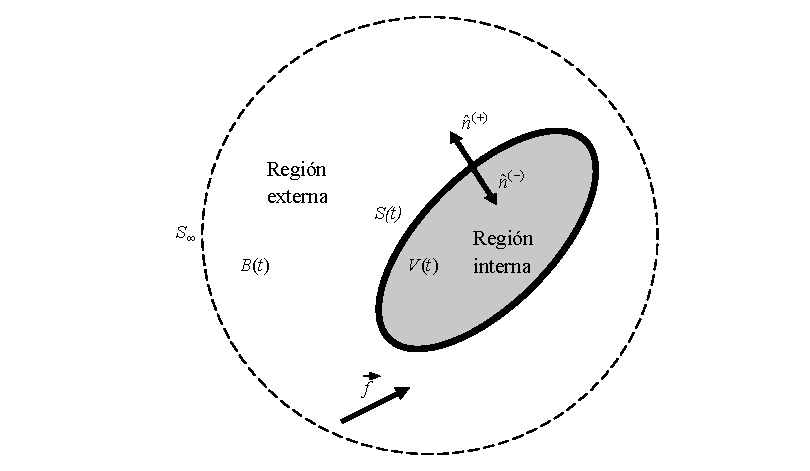
\includegraphics[width=5.0 in]{infinite.pdf}
	\caption{Medio continuo interactuando con un espacio infinito.}
	\label{infinite}
\end{figure}

En el problema planteado, tanto las variables {\bf fuente} como las variables
{\bf causa} se encuentran conectadas en términos discretos a través de una ley
como la indicada en \cref{ca_ef}. Ya señalamos que para tratar estas variables de carácter discreto  como una función, se procede partiendo del concepto de límite.  Para esto supondremos que realizaremos particiones del medio continuo en celdas de volumen (cada una de las cuales será también un sistema de infinitas partículas dado que se ha despreciado la microestructura a todas las escalas) y que para eliminar la dependencia del tamaño de la partición daremos a estas celdas un tamaño cada vez más pequeño hasta alcanzar un estado límite en el cual supondremos que cada celda se convierte en lo que denominaremos por ahora un punto material para diferenciarlo del punto matemático.  Es decir a la celda de volumen de la \cref{material} le estamos asignando material.

\begin{equation}
\mathop {\lim }\limits_{\Delta V \to 0} \Delta V = Punto\; {\rm{ material}}
\label{material}
\end{equation}

\begin{itemize}
\item A la luz de la continuidad matemática el punto material definido en la \cref{material} no posee tamaño.  Este sin embargo encierra o esta conformado por infinitas partículas; es decir, el punto material es a la vez un medio continuo.

\item Matemáticamente dicho punto siempre existe, esta es la hipótesis básica de
continuidad.  Físicamente en el proceso de cálculo del límite dado en la
\cref{material} eventualmente se alcanzará un tamaño finito donde la hipótesis de continuidad comienza a colapsar y el límite deja de ser válido; a partir de este tamaño el efecto de la micro-estructura despreciada desde el inicio comienza a ser importante y en el límite eventualmente la celda se convierte en una de las partículas de la micro-estructura.  De hecho, podría convertirse en un vacío.

\item Si las dimensiones características del espécimen son varios órdenes de
magnitud mayores que este tamaño límite finito, siempre será valido trabajar con
la definición matemática de punto, \cref{material}.  Es decir si el $\Delta V$
físico es menor en varios órdenes de magnitud que todas las dimensiones
importantes del sistema de infinitas partículas será válida la hipótesis de
continuidad física dada en la \cref{material}.
  
\end{itemize}

Regresemos nuevamente al nivel de la {\bf partícula} y mantengamos la
designación de $\alpha$ para la variable {\bf fuente} o {\bf causa} que aparece de forma explícita en asocio con una partícula y la cual produce cambios de una variable tipo {\bf efecto} o {\bf respuesta} $\beta$. Deseamos considerar esta variable como una distribución o función en el medio continuo.  Denotaremos esta función resultante como $\Phi$.  Esta puede ser de carácter escalar, vectorial o en general tensorial.  Recordemos además que las variables $\alpha$ y $\beta$ están relacionadas mediante una ley general o principio fundamental;

\begin{equation}
f\left( {\frac{{d\beta }}{{dt}}} \right) = \alpha
\label{ca_ef_2}
\end{equation}

El tratamiento propuesto en la \cref{ca_ef_2} necesariamente nos lleva a tener
que promediar la variable $\alpha$ sobre las celdas de volumen, es decir a
asociarlas al punto, vía el concepto de límite implicado en el cálculo
diferencial. Por ejemplo, supondremos que a una celda volumétrica finita $\Delta
{V_1}$ le corresponde un $\Delta {\alpha _1}$, a una celda inferior $\Delta
{V_2}$ un $\Delta {\alpha _2}$ y así sucesivamente de manera tal que en el estado límite del punto en el sentido de \cref{material} la relación $\Delta \alpha /\Delta V$ tenderá a una función continua $\Phi$ y que en el punto material asume por lo tanto un valor constante.

\begin{equation}
\mathop {\lim }\limits_{\Delta V \to 0} \frac{{\Delta \alpha }}{{\Delta V}} = \Phi
\label{distri}
\end{equation}

\begin{itemize}
\item En \cref{distri} $\Delta V$ tiende a cero mientras que la relación $\Delta \alpha /\Delta V$ se asume aproximándose al valor dado $\Phi$.

\item El límite de la \cref{distri} no ha sido calculado a través de ningún
procedimiento matemático explícito sino que su existencia se impone en el modelo como hipótesis de partida.  Es decir se asume la existencia de dicho límite.

\item El proponer la existencia del límite dado por la \cref{distri} ha sido
motivado por la hipótesis de continuidad física y su relación directa con el continuo matemático. En estos términos la existencia de dicho límite podría entenderse como un postulado fundamental sobre el cual se está construyendo el modelo del medio continuo. 

\item Si los resultados del modelo construido a partir del límite dado en
\cref{distri} logran predecir las observaciones experimentales entonces el modelo resultante habrá sido exitoso, en caso contario este debe ser enriquecido, mejorado o en el caso extremo abandonado.  Por ejemplo si $\Phi$ en \cref{distri} no asume un valor constante sino una variación (por ejemplo lineal) entonces será posible capturar fluctuaciones lineales (o localizaciones) de $\Phi$ en el punto material.  Este principio podría seguirse extendiendo para considerar fluctuaciones más fuertes como por ejemplo cuadráticas y de orden superior, hasta que eventualmente se alcanzaría un nivel de refinamiento comparable en términos de precisión con un resultado discreto.  Lógicamente, en la medida en que se aumenta el orden de la fluctuación asumida sobre el punto material aparecen cada vez más ecuaciones.

\item Finalmente, la nueva función $\Phi$ estará asociada con un punto material en el sentido de la \cref{material} y se tratará ahora como una cantidad de $\alpha$ por unidad de volumen que varia de manera continua a lo largo de $V(t)$, es decir como un campo.  Se dice entonces que la función $\Phi$ representa una densidad volumétrica de $\alpha$ .  Cuando son vistas en asocio con una superficie estas densidades se convierten en densidades superficiales; cantidad de $\alpha$ por unidad de superficie.

\end{itemize}

En la \cref{macromicro} se esquematiza un problema para un espécimen
uni-dimensional de tamaño $L$.  La escala de tamaño del espécimen se denominará en lo que sigue la macro-escala.  En ésta, una función del tipo $\Phi$ varía a lo largo del dominio matemático ocupado por el sistema de partículas o puntos materiales.  En un punto material cualquiera del dominio $L$, la variable $\Phi$ asume un valor constante de manera consistente con el límite dado en la \cref{material}. Sin embargo ya es claro que físicamente sobre el punto material se presentan o existen entes de carácter discreto y sobre los cuales las variables presentan fuertes fluctuaciones.  Por ejemplo en el inserto de la \cref{macromicro} se denota por $\ell$ la escala de tamaño sobre la cual se presentan las fluctuaciones.  Este dominio se denominará en lo que sigue la micro-estructura.  En esta misma figura se esquematiza también mediante la línea punteada el valor promedio de las fluctuaciones y correspondiente al valor constante asignado en el punto material de la parte superior de la Figura.  Como conclusión las fluctuaciones asociadas con la micro-estructura o carácter discreto de la materia no serán capturadas por el modelo del continuo válido sobre el dominio o a la escala de tamaño $L$.

\begin{figure}[H]
\centering
	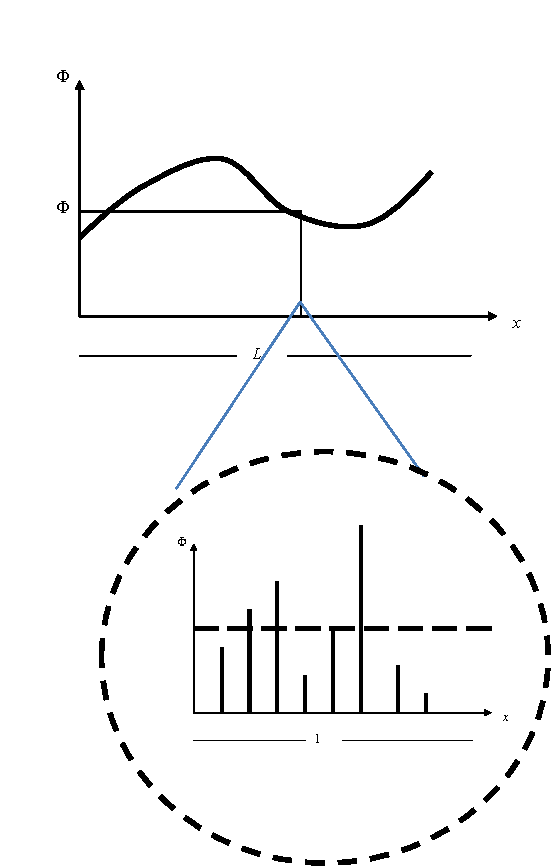
\includegraphics[width=3.0 in]{macromicro.pdf}
	\caption{Dominio del Medio Continuo representando la Macro-escala y la micro-escala.}
	\label{macromicro}
\end{figure}


A través del concepto del límite establecido en \cref{material} lo que se hace entonces es asignar al volumen o punto material matemático el valor promedio acomodado sobre el punto o volumen material físico.  En estos términos es claro que la distribución de la función $\Phi$ a nivel macro representa una aproximación con respecto a la distribución a nivel micro.  Las predicciones a nivel del continuo basado en la \cref{material} serán válidas mientras se de la condición $L \gg \ell $.

Más aún, nos referiremos al volumen o punto material físico (como el de la parte superior de la \cref{macromicro}) como Volumen Representativo del Material (VRM).  De acuerdo con esto se tiene entonces que un continuo clásico puede entenderse como una variedad \footnote{Variedad o en Ingles la denominada Manifold.  Correspondiente a una estructura topológica} de puntos materiales abstractos o Volúmenes Representativos del Material.

De acuerdo con la hipótesis de continuidad matemática estos puntos materiales a la vez están conformados por un número infinito de puntos materiales de manera que matemáticamente o por abstracción siempre será posible seguir descendiendo en tamaño sin nunca encontrar los entes micro-estructurales o de tipo discreto.  Sin embargo en otros modelos del continuo (denominados como no-clásicos) el VRM puede ser dotado de alguna capacidad de describir (aunque aún en términos del continuo) cierto tipo de fluctuaciones micro-estructurales.  Más adelante se hará referencia a este tipo de propuestas.

\section*{Volumen Representativo del Material \footnote{Algunos casos de determinación del VRM se presentan en las referencias \cite{bonda1996effect,bonda1992deformation}.}}


Habiendo identificado el VRM como el bloque constitutivo fundamental de un
modelo del medio continuo es útil en esta sección dar un poco más de precisión
a esta definición.  Para esto se presentan algunas micro-estructuras relativas y se reitera sobre la manera de producir un continuo clásico en términos de asignaciones de variables a puntos materiales abstractos e ideales correspondientes a valores promedios calculados sobre puntos materiales físicos e identificables en el laboratorio.

De la discusión precedente es claro que implícita en la estrategia utilizada en la hipótesis básica de continuidad se encuentra un proceso de homogenización o transición de menor a mayor escala de tamaño.  Por homogenización nos referimos a la asignación de propiedades físicas a los puntos materiales correspondientes a un promedio de los valores asumidos por varias partículas sobre un volumen finito de material.

Como ya se mencionó y de acuerdo con postulados fundamentales de la mecánica cuántica los sistemas formados por átomos, electrones, protones, neutrones y partículas subatómicas carecen de continuidad.  Es decir, a este nivel no se logra una precisión aceptable si se opera bajo la hipótesis de continuidad.

En la dirección ascendente en cuento a tamaño el siguiente nivel de fragmentación se identifica en la molécula.  La mecánica clásica de los medios continuos ha sido construida sobre la hipótesis de que a este nivel efectivamente se logran resultados con la precisión adecuada y de que por encima de este nivel no existen otros entes micro-estructurales.  Es decir, para volúmenes de tamaños iguales y superiores a la molécula las aproximaciones basadas en la hipótesis básica de continuidad usadas en la mecánica clásica permitirían llegar a resultados aceptables.

Sin embargo desarrollos relativamente recientes, motivados por las nuevas tendencias hacia la miniaturización, han revelado escalas de tamaño varios órdenes de magnitud superior a la escala molecular donde la mecánica clásica también comienza a agotar su nivel de precisión.  Este es el caso particular de los denominados materiales con micro-estructura.  De lo anterior se desprende el hecho de que existe un volumen mínimo de material por debajo del cual es impreciso abordar el problema de las infinitas partículas a partir de la hipótesis básica de continuidad.  Desde el punto de vista matemático dicho volumen será siempre considerado infinitamente pequeño.

Pudiéramos pensar en esta escala como la correspondiente a la microestructura
del material a través de la cual seria posible identificar de manera discreta
vacíos, impurezas, defectos o en general heterogeneidades.  Supongamos que en esta escala las heterogeneidades se encuentran separadas a unas distancias promedio $\ell$  (la micro-escala definida en la sección anterior).  Por ejemplo, consideremos un volumen de material de tamaño característico comparable a esta distancia $\ell$.  Es claro que si se estuviera analizando un espécimen con dimensiones características $L$ (la macro-escala) cercanas o comparables con $\ell$ la validez de un tratamiento con base en la hipótesis de continuidad sería fácilmente cuestionable pues se generarían fluctuaciones como las de la \cref{macromicro}.  La \cref{solder} ilustra una de estas microestructuras correspondiente a una aleación plomo/estaño en la cual la separación de los defectos es del orden de $5.0 \mu m$.  Si se estuviera analizando vía la mecánica del medio continuo un espécimen con un tamaño cercano al de estas micro-estructuras, los resultados no capturarían concentraciones de las variables del tipo $\Phi$ sobre las diferentes fases, por ejemplo sobre la fase de plomo o de estaño.  La pregunta es entonces: ¿a partir de que tamaño $L$ del espécimen es válido comenzar a suponer que efectivamente se tiene un comportamiento representable como un medio continuo?.  En otras palabras, a partir de que tamaño $L$ es válido afirmar que si se divide el medio en celdas infinitesimales a las cuales se les confieren propiedades mecánicas promedio, las predicciones del modelo estarán dentro de rangos de precisión aceptables desde el punto de vista de la ingeniería?

\begin{figure}[H]
\centering
	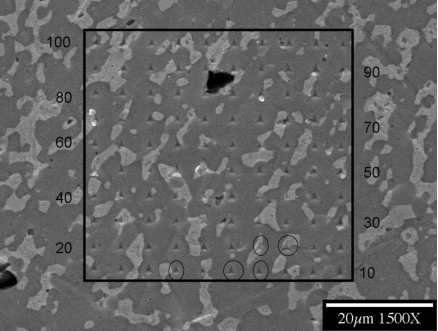
\includegraphics[width=2.5 in]{solder.pdf}
	\caption{Fotografía aumentada de una aleación de plomo/estaño utilizada en aplicaciones de microelectrónica.}
	\label{solder}
\end{figure}

La respuesta depende claramente del tipo de micro-estructura inherente en cada material.  En los desarrollos tempranos de la mecánica del medio continuo el problema fue evadido asumiendo que se estaba a escalas varias veces por encima de las distancias intra-moleculares despreciando la existencia de entes fundamentales de tamaño superior.  Aunque para la ingeniería clásica este modelo del medio continuo ha resultado ser lo suficientemente preciso, el desarrollo de tecnologías e industrias emergentes \footnote{Como por ejemplo la micro-electrónica y la nano-tecnología} ha empezado a llevar al modelo al límite de su precisión.  En esta presentación se llama la atención sobre la existencia de esta escala inferior por debajo de la cual no sería válido proceder vía el continuo y se introduce el concepto de volumen representativo del material como una propiedad mecánica adicional cuyo valor depende de cada material.  Claramente esta propiedad $\ell$ tiene dimensiones de longitud y varía de material a material y de microestructura a microestructura.

En lo que sigue asumiremos que el sistema de infinitas partículas (no
necesariamente todas iguales) estará ocupando un espacio físico de manera continua (en el sentido físico y matemático), o equivalentemente se asumirá continuidad de puntos y de partículas; \textbf{\textit{entre dos partículas del sistema, sin importar que tan cercanas se encuentren siempre será posible asignar otra partícula.}} En otras palabras se le está confiriendo acá a la partícula el carácter de punto material.  Este espacio se subdividirá en volúmenes infinitesimales $\Delta V$ a cada uno de los cuales se les conferirán propiedades (mecánicas) constantes.  Nos referiremos a este volumen como \textbf{Volumen Representativo del Material  (VRM)} \footnote{VRM: Mínimo volumen sobre el cual el material es estadísticamente homogéneo,$F(x)=x$}.  Asumiremos además que siempre estaremos operando en especímenes con tamaños superiores a este VRM y que estaremos haciendo mediciones a escalas igualmente superiores.  La presencia de la microestructura y de un punto material físico o VRM se esquematiza en la \cref{VRM}.  Cabe anotar que la ingeniería moderna ha reconocido la potencia práctica de la hipótesis del medio continuo como herramienta de solución de problemas y ha planteado modelos que intentan ampliar las capacidades del mismo a escalas bastante cercanas a las del VRM.  Estas se han denominado como teorías no-locales, de cinemática enriquecida o simplemente teorías no-clásicas de la mecánica de los medios continuos. \footnote{Algunas de estas son las propuestas por Voigt, W(1887).  Theoretische Studien uber die Elastizitatsverhaltnisse der Krystalle.  Abh. Koniglichen Gesellschaft Wiss.  Gottingen., Cosserat, E., and Cosserat, F(1909).  Theorie des Corps Deformables.  Paris: A Hermann \& Fils., Aero, E., Kuvshinsky, E(1961).  Fundamental equations of the heory of elastic media with rotationally interacting particles.  Soviet Physics Solid State.  Vol 2.  pp 1272., Eringen, A.C(1968).  Theory of Micropolar Elasticity.  In Fracture, and advanced treatise.  Eds Leibowitz, H.  Academic Press, New York, pp 621-729., Mindlin, R(1964).  Micro-structure in Linear Elasticity.  Arch. Ration. Mech. Anala.  Vol 16, pp 51-78., Toupin, R(1962).  Elastic Materials with Couple-Stresses.  Arch.Rational Mech.Anal.  Vol 11, pp385-414.}.

\begin{figure}[H]
\centering
	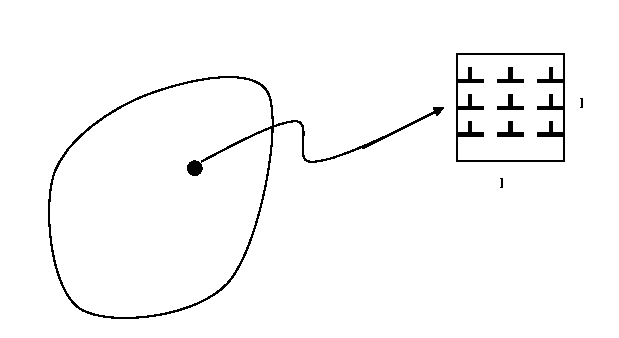
\includegraphics[width=3.0 in]{VRM.pdf}
	\caption{Esquematización del Volumen Representativo del Material y de las macro y meso-escalas.}
	\label{VRM}
\end{figure}

Con base en las discusiones anteriores, estos modelos no-clásicos lo que hacen es dotar al VRM de información referente a la micro-estructura en términos de variables que varían de manera continua, como por ejemplo parámetros relativos a su tamaño, que permiten describir distribuciones no-constantes localizadas al interior del punto material matemático lo que permite dar cuenta en términos del continuo de fluctuaciones no capturables por una propuesta clásica.

\section{Conceptos Preliminares}
Antes de presentar el método general que se utilizará para reducir las variables discretas a distribuciones, densidades o campos es necesario introducir algunos conceptos preliminares.

\subsection{Hipótesis Básica de Continuidad}
Aunque la descripción de los cambios de configuración a los cuales se puede someter un medio continuo se estudiará de manera formal y detallada en secciones posteriores, será útil hacer acá una referencia inicial a este respecto, en particular en lo concerniente con la descripción del movimiento en el caso de un medio deformable.  En este sentido resultará útil y común comparar las configuraciones, localizaciones o lugar geométrico de las infinitas partículas del sistema en dos instantes.

\begin{itemize}
\item Un instante o configuración inicial que denotamos como correspondiente a $t=0$ , donde $t$ representa un marco de referencia temporal.  Nos referiremos a esta configuración indistintamente como el medio continuo en $t=0$, \textit{la configuración de referencia o la configuración no-deformada}.  Se asumirá que en esta configuración el medio continuo se encuentra libre de interacciones con el medio ambiente.

\item Un instante o configuración posterior $t=t$.  Nos referiremos a esta configuración indistintamente como el {\bf medio continuo} en $t=t$, \textit{la configuración actual o la configuración deformada}.  Se asume que el medio continuo es llevado a esta configuración precisamente por la acción de interacciones externas. 

\end{itemize}

Al comparar estas dos configuraciones se asumirá que en ambos estados la
cantidad de materia es la misma.  Más aún, siguiendo un enfoque causa-efecto supondremos que es la acción de las interacciones externas la que produce los cambios de configuración entre $t=0$ y $t=t$.

La hipótesis básica de continuidad desde el punto de vista físico consiste en suponer que las infinitas partículas que conforman el sistema ocupan o llenan de manera continua un espacio físico determinado de volumen $V$ y acotado por una superficie o frontera $S$.  Esta hipótesis física permite ahora representar todas las propiedades como funciones continuas y posibilita el uso del cálculo como herramienta matemática.  Más adelante se identificarán algunas consecuencias de esta hipótesis básica.


\subsection{Partícula o Punto Material}
En el contexto de la mecánica de los medios continuos por partícula o punto material se estará haciendo referencia a cantidad de materia o porción infinitesimal de un cuerpo pero sin conceder a esta geometría alguna tal y como se estipula en el límite dado en la \cref{material}.  Tampoco se detalla ésta es un átomo, molécula o que tipo de ente fundamental.  A pesar de la carencia de geometría la partícula tendrá siempre asociado un volumen y una densidad de masa.  Esta contradicción aparente es una consecuencia del uso del concepto matemático de límite.  El punto material podrá experimentar desplazamiento, velocidad, aceleración, cambios de momentum o en general flujos e interacciones.  El punto material se considerará como el elemento constitutivo primario o elemental de un modelo de los medios continuos.

\subsection{Punto}
Por punto se hará referencia a una localización geométrica fija con respecto a un sistema de referencia.  El punto como tal tampoco posee geometría alguna y mucho menos tendrá asociadas cantidades físicas.  Sin embargo, en un instante dado, un punto puede estar siendo ocupado por un punto material con propiedades físicas asociadas.  En este caso hablaremos de la propiedad en el punto pero teniendo en cuenta que en realidad esta será debida a la contribución del punto material.  Más aún, pueden existir interacciones del punto con el medio externo de manera tal que cuando una partícula ocupa este punto, está siente una contribución adicional o agente modificador de sus propiedades.

\subsection{Cuerpo}
Nos referimos a un cuerpo como un sistema de infinitas partículas (ahora puntos materiales) lo cual no constituye ninguna novedad ya que en cursos básicos de física se había trabajado con el caso de cuerpos rígidos.  Se trataba precisamente de un sistema de infinitas partículas pero en este caso el apelativo de cuerpo rígido hacía referencia al hecho de que las distancias intra-particulares antes y después de la consideración de las fuerzas permanecían constantes.  Claramente esta hipótesis permitía abordar el problema sin la necesidad de hacer referencia alguna al material constitutivo y permitía tratarlo como una partícula con la adición de la interacción rotacional.

En lo que sigue se liberará la hipótesis anterior y se asumirá que como resultado de las interacciones del sistema con el medio ambiente este puede exhibir cambios en las distancias intra-particulares.  La magnitud de estos cambios dependerá en cada caso de la naturaleza de las fuerzas inherentes que le dan el carácter denso al sistema, es decir enlaces electroquímicos, electromagnéticos, etc.  En otras palabras a igual intensidad de fuerzas aplicadas a cuerpos de igual geometría pero de materiales diferentes los cambios en distancias entre partículas dependerán del material del cuerpo.  Los cambios en las distancias intra-partícula se reflejarán posiblemente no solo en cambios de posición sino también de forma y de tamaño del cuerpo.  Uno de los propósitos del modelo de la mecánica del medio continuo es caracterizar o describir estos cambios a nivel local o del punto material definido este en el sentido de la \cref{lim_point} en la sección introductoria.

\end{document}


